\usetheme{Berlin}
\usecolortheme{beaver}

\usepackage[utf8]{inputenc}
\usepackage[T1]{fontenc}
\usepackage{lmodern}

\usepackage{graphicx}
\usepackage{float}
\usepackage{caption}
\captionsetup{labelformat=empty,labelsep=none}

\usepackage{color}
\newcommand{\hilight}[1]{\colorbox{yellow}{#1}}

\newcommand{\norm}[1]{\lVert#1\rVert}

\title{Intermediate presentation\\
Gilbert: A sparse linear algebra environment}
\author[T. Rohrmann]{Till Rohrmann\\
\texttt{till.rohrmann@campus.tu-berlin.de}}
\institute[TUB]{Technische Universität Berlin}
\date{\today}
\subject{Gilbert: A sparse linear algebra environment}

\begin{document}
		\frame{\titlepage}
		\begin{frame}
			\frametitle{Table of Contents}
			\tableofcontents
		\end{frame}
		%!TEX root = presentation.tex
\section{Motivation}

\begin{frame}
	\frametitle{Big data analytics}
	\begin{columns}
		\begin{column}{0.6\textwidth}
			\begin{itemize}
				\item Gathered data grows exponentially
				\item Obtain new insights
				\item Analytic methods have to scale up $\Rightarrow$ Parallelization
				\item Methods developed within linear algebra systems
				\item Explicit parallelization tedious and error-prone
			\end{itemize}
		\end{column}
		\begin{column}{0.4\textwidth}
			
\includegraphics[width=\textwidth]{images/bigData.jpg}
		\end{column}
	\end{columns}
\end{frame}

\begin{frame}
	\frametitle{Distributed computing and data analytics}
	\begin{columns}
		\begin{column}{0.6\textwidth}
			\begin{itemize}
				\item Experts familiar with both domains countable
				\item Laborious to become acquainted with new domain
				\item Huge existing code base
				\item Can't we bring both worlds together?
				\item Solution: Gilbert
			\end{itemize}
		\end{column}
		\begin{column}{0.4\textwidth}
			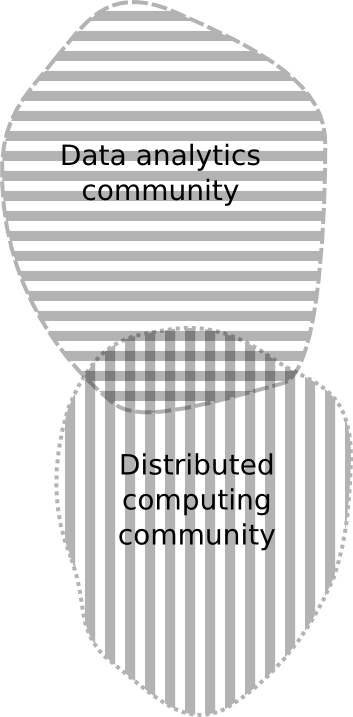
\includegraphics[height=0.8\textheight]{images/intersection.png}
		\end{column}
	\end{columns}
\end{frame}
		%!TEX root = presentation.tex
\section{Gilbert}

\begin{frame}
	\frametitle{Gilbert}
	\begin{itemize}
		\item Sparse linear algebra system
		\item Matlab frontend for distributed computing frameworks
		\item Allows to almost seamlessly move from local execution to distributed execution in a heterogenous environment
		\item Enable machine learning and data analytics algorithms to be run distributedly
	\end{itemize}
\end{frame}
		%!TEX root=presentation.tex
\section{Approach}

\begin{frame}
	\frametitle{Approach}
	\begin{columns}
		\begin{column}{0.6\textwidth}
			\begin{enumerate}
				\item Compiling Matlab code into intermediate representation
				\item Apply optimizations indenpendently of runtime specific system
				\item Compiling intermediate representation into runtime specific format
			\end{enumerate}
		\end{column}
		\begin{column}{0.4\textwidth}
			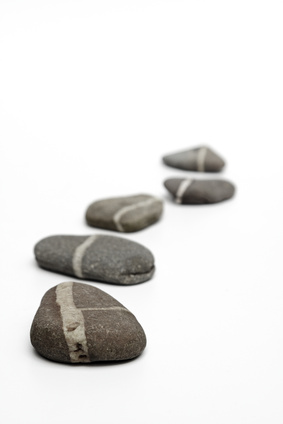
\includegraphics[width=0.8\textwidth]{images/approach.jpg}
		\end{column}
	\end{columns}
\end{frame}

\begin{frame}
	\frametitle{System architecture}
	\begin{center}
		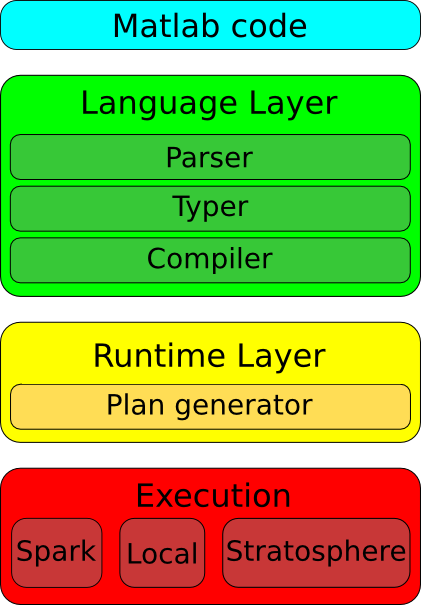
\includegraphics[height=0.8\textheight]{images/architecture.png}
	\end{center}
\end{frame}

\begin{frame}[fragile]
	\frametitle{Language}
	\begin{columns}
		\begin{column}{0.60\textwidth}
			\begin{itemize}
				\item Matlab-like language
				\item Support of basic linear algebra operations
				\item Some built-in functions, repmat, linspace, pdist2
				\item Loop support with static and dynamic termination criterion
				\item Language expressive enough to support variety of algorithms, Pagerank, K-means, NNMF
			\end{itemize}
		\end{column}
		\begin{column}{0.4\textwidth}
			\begin{lstlisting}[basicstyle=\scriptsize, numbers=left, stepnumber=2]
A'*B

f = @(x) x.^2.0

eps = 0.1

c = @(p,c) norm(p-c,2) < eps

fixpoint(1/2, f, 10, c)
			\end{lstlisting}
		\end{column}
	\end{columns}
\end{frame}

\begin{frame}
	\frametitle{Compilation: Intermediate format}
	\begin{itemize}
		\item Scala's combinator parsing tool box
		\item Powerful enough for our language
		\item Matlab is dynamically typed
		\item Execution on Stratosphere requires type knowledge at compilation time
		\item Hindley-Milner type inference algorithm to infer types and dimensions
	\end{itemize}
\end{frame}

\begin{frame}[fragile]
	\frametitle{Example: Parsing and typing}
	\begin{block}{Input}
\begin{lstlisting}[language=Matlab]
A = ones(2,10);
B = eye(10,3);
A*B
\end{lstlisting}
\end{block}
	
\begin{block}{Parsed and typed}	
\begin{lstlisting}[language=Matlab]
A = ones(2,10):MatrixType[Double,2,10];
B = eye(10,3):MatrixType[Double,10,3];
A*B:MatrixType[Double,2,3]
\end{lstlisting}
\end{block}

\end{frame}

\begin{frame}[fragile]
	\frametitle{Example: Intermediate code}
	\begin{block}{Compiled}
\begin{lstlisting}[columns=flexible, language=Java]
MatrixMult(
  ones(
    IntValue(2),
    IntValue(10)
  ), 
  eye(
    IntValue(10),
    IntValue(3)
  )
)
\end{lstlisting}
	\end{block}
\end{frame}

\begin{frame}
	\frametitle{Example: Stratosphere execution plan}
	\begin{center}
		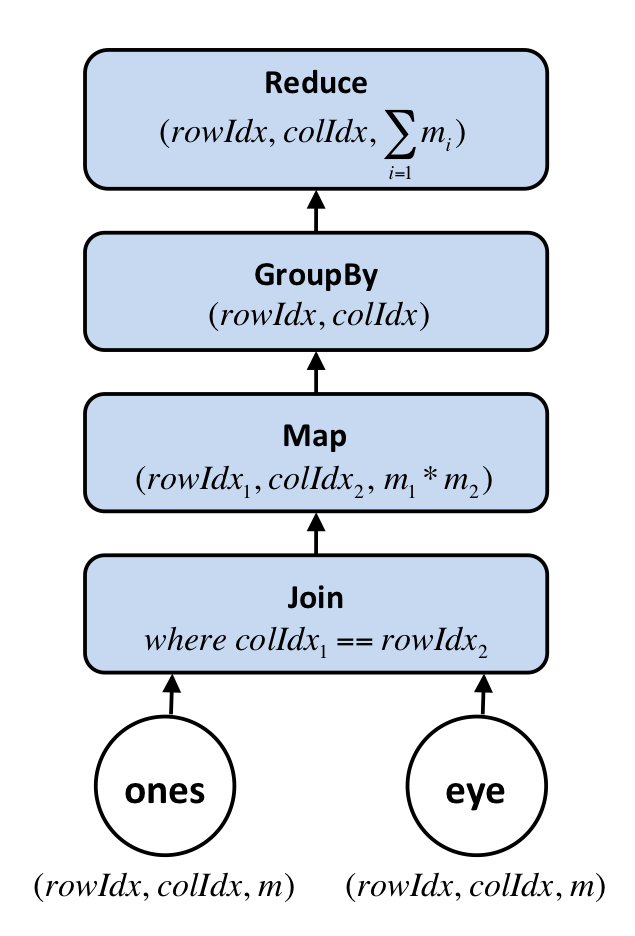
\includegraphics[height=0.85\textheight]{images/matrixMultDataflow.png}
	\end{center}
\end{frame}
		\section{Current state}

\begin{frame}
	\frametitle{Current state}
	\begin{itemize}
		\item Language layer working (except for the typing algorithm which is still a little bit buggy)
		\item Execution on Stratosphere with iteration and convergence support
		\item PageRank, NNMF and K-means executable
	\end{itemize}
\end{frame}

\begin{frame}
	Live demonstration
\end{frame}		
		\section{Outlook}

\begin{frame}
	\frametitle{Outlook}
	\begin{itemize}
		\item Implement typing system with constraints, e.g. Haskell typing system with type class support
		\item Evaluate implementation: Runtime, scalability
		\item Compare to specialized algorithms
		\item Implement optimizations for the intermediate representation
	\end{itemize}
\end{frame}
		\nocite{*}
\begin{frame}[noframenumbering,plain,allowframebreaks]{References}
	\frametitle{Bibliography}
	\printbibliography
\end{frame}
\end{document}
